\documentclass[a4paper, oneside]{book}

\usepackage{geometry,url,graphicx, hyperref,subfig,enumitem}
\usepackage{amsmath, amssymb, amsthm, mathtools, color, setspace}
\usepackage{fancyhdr, braket, etoolbox}
\usepackage{xfrac, lmodern} % xfrac gives font errors, add lmodern to remove them. Check whether this remains a problem!
%\usepackage{hyperref}
%\usepackage[utf8]{inputenc}
%\usepackage{colorprofiles}
\usepackage[T1]{fontenc}

\begin{document}
	\begin{titlepage}
		%%%% LOGO %%%%
		\begin{figure}
			
\includegraphics[width=\linewidth]{tesi_images/logo.jpg}
		\end{figure}
		\center
		\textsc{\large Corso di laurea in Fisica}\\[0.2cm]
		\textsc{\normalsize Tesi di laurea triennale}\\[2cm]
		%\rule{\linewidth}{0.3mm} \\[1.2cm]
		
		% TITLE
		\begin{doublespace}
			\textbf{\LARGE A machine learning approach to the electrons and photon classification with the ATLAS detector at the LHC}
			\\[2cm]
		\end{doublespace}
		
		% AUTHOR
		\begin{minipage}{0.4\textwidth}
			\begin{flushleft}
				\emph{Autore:} \\[0mm]
				\textbf{Pietro Daniele} \\[4mm]
				\emph{Matricola:}\\
				906962 \\[4mm]
				\emph{Codice P.A.C.S.:}\\[0mm]
				07.05.-t
			\end{flushleft}
		\end{minipage}
		%
		\begin{minipage}{0.4\textwidth}
			\begin{flushright} 
				\emph{Relatore:} \\
				\textbf{Prof. Leonardo Carlo Carminati} \\[1.2em]
				\emph{Corelatori:} \\
				\textbf{Dott. Ruggero Turra} \\
				\textbf{Dott. Davive Mungo} \\[1.2em]
			\end{flushright}
		\end{minipage}\\[2cm]
		\vfill
		Anno accademico 2019-2020
		
	\end{titlepage}

\tableofcontents

	\chapter{LHC and ATLAS}
		\section{The LHC}
		The CERN Large Hadron Collider is a two-ring, superconducting accelerator and collider installed in the long LEP tunnel (27 km)\cite{LHC design} and it provides pp collisions and heavy-ion (e.g. Pb-Pb) collision.\\
		Inside the accelerator, two high-energy particle beams travel at close to the speed of light before they are made to collide. The beams travel in opposite directions in separate beam pipes (two tubes kept at ultrahigh vacuum). They are guided around the accelerator ring by a strong magnetic field maintained by superconducting electromagnets\cite{LHC introduction}
			\subsection{Lattice Layout}
			\begin{figure}
				\centering
				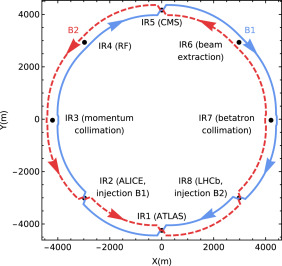
\includegraphics[width=0.3\textheight]{tesi_images/LHC_structure.jpg}
				\caption{LHC structure}
			\end{figure}
			The basic layout of the LHC follows the LEP tunnel geometry. The LHC has eight arcs and straight sections. Each straight section is approximately 528 m long and can serve as an experimental or utility insertion. The two high luminosity experimental insertions are located at diametrically opposite straight sections: the ATLAS experiment is located at point I and the CMS experiment at point 5.\\
			Two more experimental insertions are located at point 2 and point 8 which also contain the injection systems for Beam
			J and Beam 2, respectively. The injection kick occurs in the vertical plane with the two beams arriving at the LHC from below the LHC reference plane. The beams only cross from one magnet bore to the other at
			these four locations.\\
			The remaining four straight sections do not have beam crossings. Insertion 3 and 7 each contain two collimation systems. Insertion 4 contains two RF systems: one independent system for each LHC
			beam. The straight section at point 6 contains the beam dump insertion where the two beams are vertically
			extracted from the machine using a combination of horizontally deflecting fast-pulsed ('kicker') magnets and
			vertically-deflecting double steel septum magnets. Each beam features an independent abort system. \cite{LHC design} \\
			The protons travel inside along th LHC ring in opposite direction. The LHC beams are controlled by superconducting magnets, which have a working temperature of 1.9 K. There are two kinds of superconducting magnets: \\
			- the superconducting dipole magnets, which thanks to a 8.33 T magnetic field drive protons along the ring (circular orbit); \\
			- superconducting quadrupole magnets, which keep the beams focused. 
			\begin{figure}
				\centering
				\subfloat[][\emph{LHC dipole}]{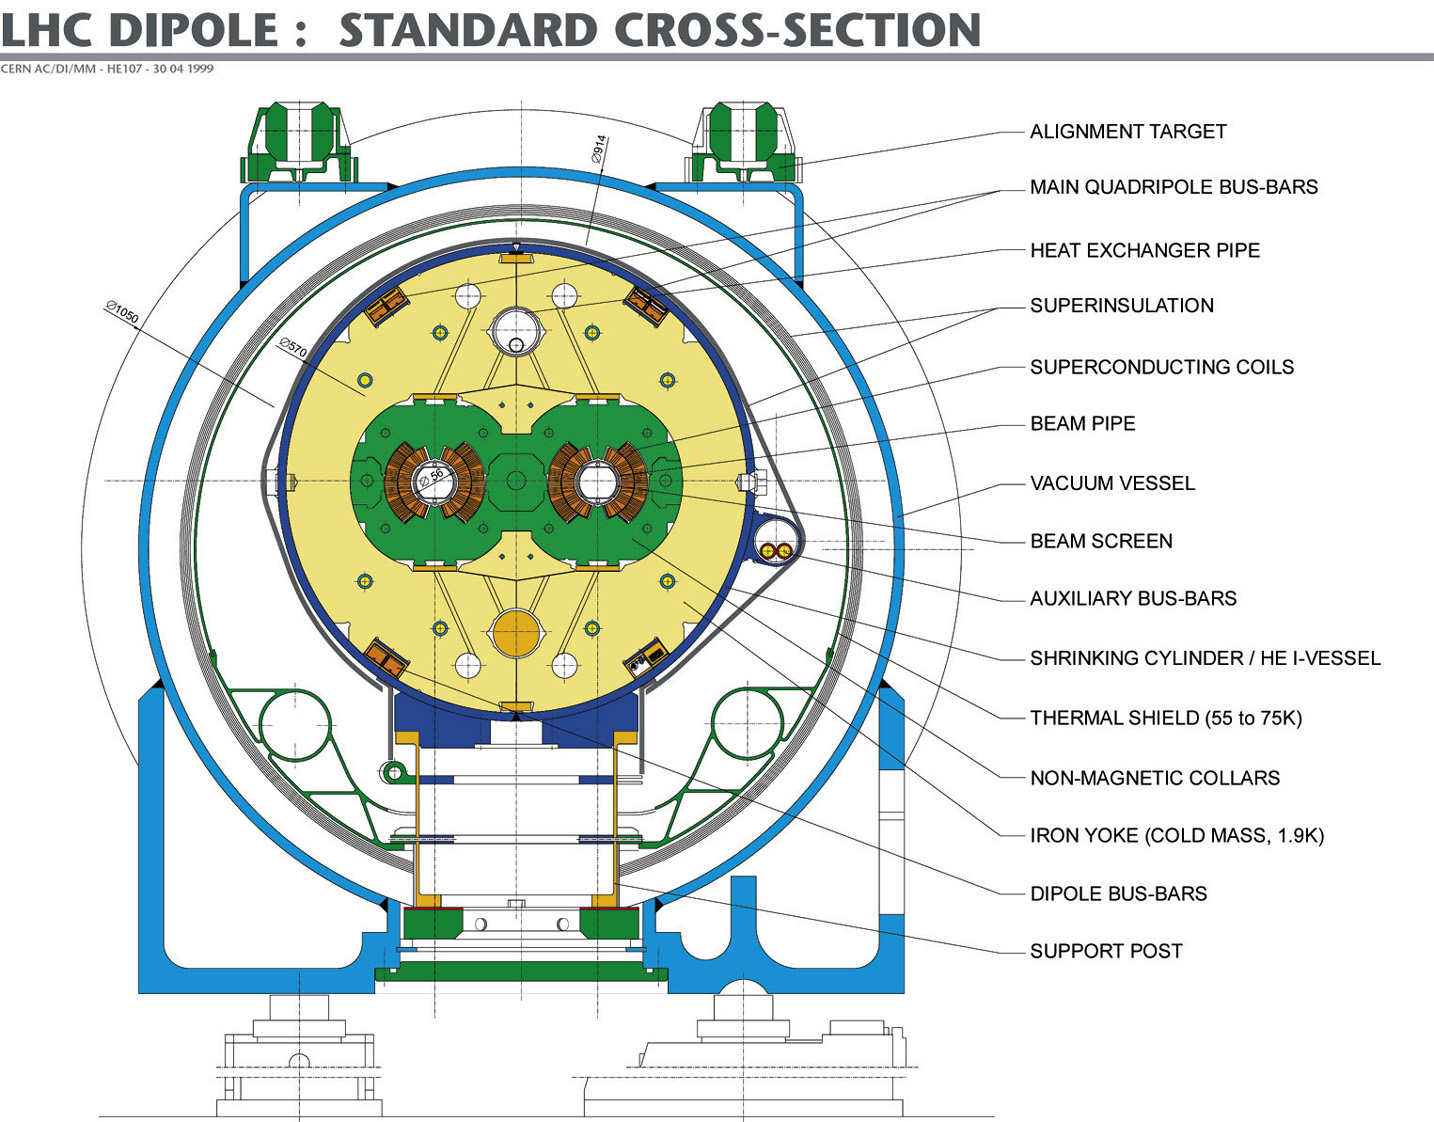
\includegraphics[width=.45\textwidth]{tesi_images/m_dipole.jpeg}} \quad
				\subfloat[][\emph{LHC quadpole}]{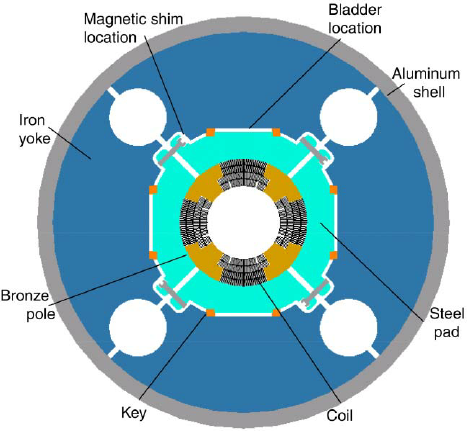
\includegraphics[width=.3\textwidth]{tesi_images/m_quad.png}} 
				\caption{LHC's superconducting magnets}
				\label{fig:subfig}
			\end{figure}
			\subsection{The CERN accelerator complex}
			Before being insert into LHC ring, particle beam is accelereted by the CERN accelerator complex. It is a succession of machins with increasingly higher energies. Each machine injects the beam into the next one, which takes over to bring the beam to an even higher energy, and so on. In  the  LHC—the  last  element  of  this  chain—each particle beam is accelerated up to the record energy of 6.5 TeV. Specifically, in LHC protons are obtained by stripping electrons from hydrogen atoms, which are taken from a bottle containing hydrogen. Then protons are injected into the PS Booster (PSB) at an  energy of 50 MeV from Linac2. The  booster  accelerates  them  to  1.4  GeV.  The  beam  is  then  fed  to  the  Proton  Synchrotron  (PS)  where  it  is  accelerated  to  25 GeV. Protons are then sent to the Super Proton Synchrotron (SPS) where they are accelerated to 450 GeV. They  are  finally  transferred  to  the  LHC  (both  in  a  clockwise  and an anticlockwise direction) where they are accelerated for 20 minutes to 6.5 TeV. Beams circulate for many hours inside the LHC beam pipes under normal operating conditions. \\
			In addition to accelerating protons, the accelerator complex can also accelerate lead ions. \cite{Acc. complex} \\
			\begin{figure}
				\centering
				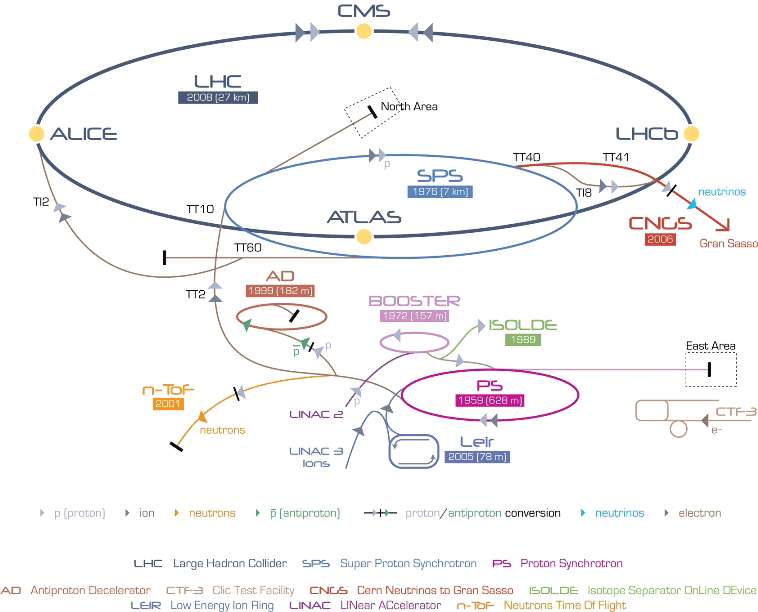
\includegraphics[width=0.3\textheight]{tesi_images/CERN.png}
				\caption{LHC and CERN's complex accelerator}
			\end{figure}
			\subsection{Proton-proton collisions}
			The numer of events per second generated in the LHC collisions is given by:
			$$
			N_{event} = L\sigma_{event}
			$$
			where $\sigma_{event}$ is the cross section for the event under study and $L$ the machine luminosity. $L$ depends only on the beam parameters and can be written for a Gaussian beam distribution as: 
			$$
			L = \frac{N_b^2n_bf_{rev}\gamma_r}{4\pi\epsilon_n\beta^*}F
			$$
			\cite{LHC design} where $N_b$ is the number of particles per bunch, $n_b$ the number of bunches per beam, $f_{rev}$ the revolution frequency, $\gamma_r$ the relativistic gamma factor, $\epsilon_n$ the normalized transverse beam emittance, $\beta^*$ the beta function at the collision point and $F$ the geometric luminosity reduction factor due to the crossing angle at the IP.
			%\footnote{ $F = \frac{1}{\sqrt{1+(\frac{\eta_c\sigma_z}{2\sigma^*})^2}}$ where $\eta_c$ is the full crossing angle at the IP, $\sigma_z$ the RMS bunch length and $\sigma_^*$ the transverse RMS beam size at the IP.}%
			
			The total inelastic proton-proton cross-section is about 80 mb at $\sqrt{s} = 14$ TeV. \cite{LHC introduction} Therefore, the event rate $R$, defined as the number of events produced per second by the pp interactions, is expected to be:
			$$
			R = \sigma L = 80 mb\times10^{34}cm^{-2}s^{-1} \simeq 10^{9}s^{-1}
			$$
			There are towo types of pp collisions:
			\begin{itemize}
				\item Soft collisions: 
				they are the most of the collisions and they are large-distance collisions between the two incoming protons. They are called "soft" because the momentum transfer of the interaction is small. Due to this feature, particle scattering at large angle is suppressed and so, after collisions, particles have a large longitudinal momentum, but small transverse momentum ($<p_T>\simeq500 Mev$) relative to the beam line. The final states
				arising from such interactions are called minimum bias events. They are not interesting.
				\item Hard collisions:
				monochromatic proton beams can be seen as beams of partons (quarks and gluons) with a wide band
				of energy. Occasionally, head-on collisions occur between two partons of the incoming protons. These are interactions at small distances, and therefore are characterised by large
				momentum transfers ("hard scattering"). In this case, particles in the final state can be produced at large angles with respect to the beam line (high $p_T$) and massive particles can be created.
				These are the interesting physics events. They are, however, rare compared to the soft interactions. \\
				In the hard-scattering interactions of quarks and gluons at a hadron collider, the effective centre-of-
				mass energy of the interaction ($\sqrt{\hat{s}}$) is, u, smaller than the centre-of-mass energy of the machine ($\sqrt{s}$) and is given by: 
				$$ 
				\sqrt{\hat{s}} = \sqrt{x_ax_bs}
				$$
				where $x_a$ and $x_b$ are the fractions of the proton momentum carried by the two colliding partons. If $x_a \simeq x_b$, then the above relation becomes
				$$ 
				\sqrt{\hat{s}} \simeq x\sqrt{s}
				$$.
				Therefore, in order to produce a particle of mass 100 GeV, two quarks (or gluons) which carry only 1\% of the proton momentum are needed ($x \sim 0.01$), whereas a particle of mass 5 TeV can only be produced if two partons with $x \sim 0.35$ interact. The momentum distributions of quarks and gluons inside the proton are called parton distribution functions. \cite{LHC introduction}
			\end{itemize}
		\section{ATLAS}	
		\cite{ATLAS intro}ATLAS is one of two general-purpose detectors at the Large Hadron Collider (LHC). It investigates a wide range of physics, from the search for the Higgs boson to extra dimensions and particles that could make up dark matter. Although it has the same scientific goals as the CMS experiment, it uses different technical solutions and a different magnet-system design.
		
		\begin{figure}
			\centering
			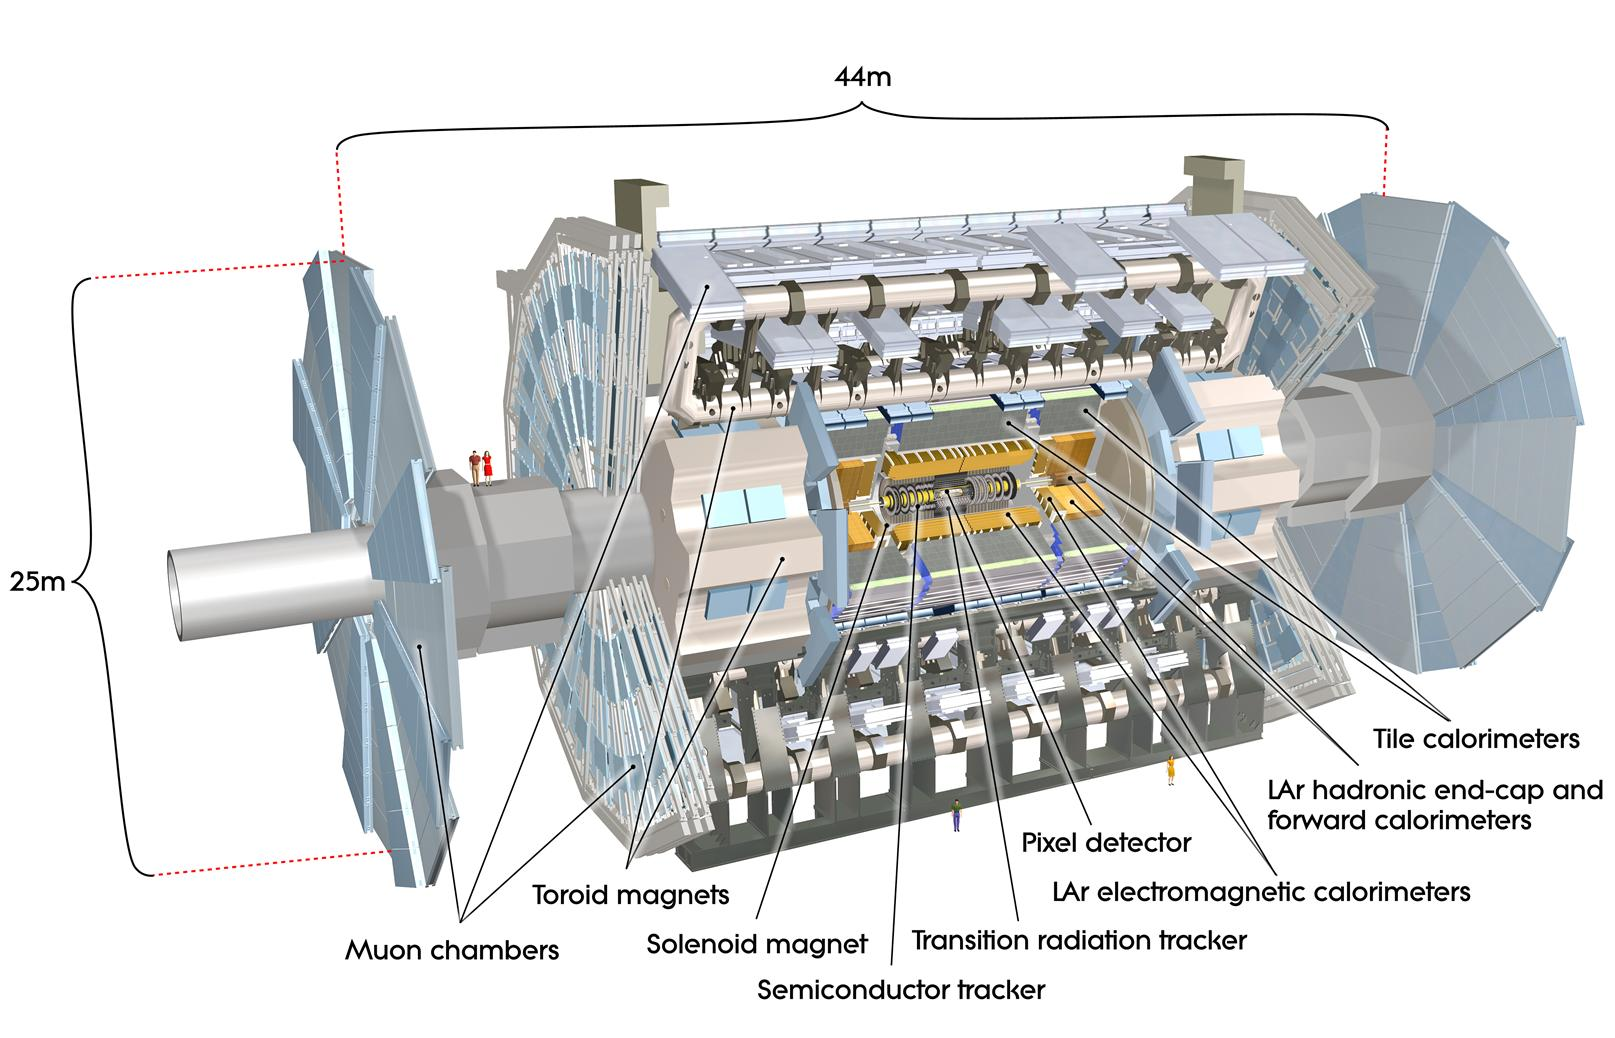
\includegraphics[width=0.45\textheight]{tesi_images/atlas_structure.jpg}
			\caption{ATLAS structure}
		\end{figure}
		
		Beams of particles from the LHC collide at the centre of the ATLAS detector making collision debris in the form of new particles, which fly out from the collision point in all directions. Six different detecting subsystems arranged in layers around the collision point record the paths, momentum, and energy of the particles, allowing them to be individually identified. A huge magnet system bends the paths of charged particles so that their momenta can be measured.
		
		The interactions in the ATLAS detectors create an enormous flow of data. To digest the data, ATLAS uses an advanced “trigger” system to tell the detector which events to record and which to ignore. Complex data-acquisition and computing systems are then used to analyse the collision events recorded. At 46 m long, 25 m high and 25 m wide, the 7000-tonne ATLAS detector is the largest volume particle detector ever constructed. 
			\subsection{Coordinate system}
			\begin{figure}
				\centering
				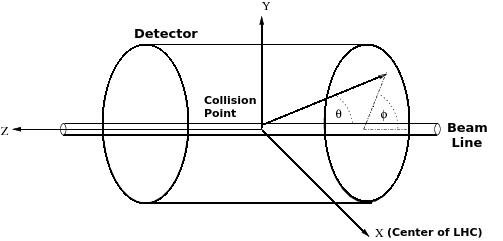
\includegraphics[width=0.3\textheight]{tesi_images/atlas_coord.jpeg}
				\caption{ATLAS coordinate system}
			\end{figure}
			\cite{ATLAS config}The origin of the coordinate system is set in the nominal point of interation. The beam direction defines the z-axis and the x-y plane is transverse to the beam direction. X-axis points from the interaction point to the centre of the LHC ring and Y-axis points upwards. The side-A of the detector is defined as that with positive z and side-C is that with negative z.
			
			Polar coordinate are also used: azimuthal angle $\phi$ is measured as usual around the beam axis, and the polar angle $\theta$ is the angle from the beam axis. Using $\theta$, pseudo rapidity is defined as $\eta= -\ln{\tan{\frac{\theta}{2}}}$. \\
			%(in the case of massive objects such as jets, the rapidity $y=\frac{1}{2}\ln{\frac{E+p_{z}}{E−p_{z}}}$ is used).%
			The transverse momentum $p_T$, the transverse energy $E_T$, and the missing transverse energy $E_T^{miss}$ are defined in the x-y plane unless stated otherwise.  The distance $\Delta R$ in the pseudo rapidity-azimuthal angle space is defined as $\Delta R = \sqrt{\Delta \eta^2 + \Delta \phi^2 }$.
			\subsection{Magnet system}
			\cite{ATLAS config}ATLAS features a unique hybrid system of four large superconducting magnets.  This magneticsystem is 22 m in diameter and 26 m in length, with a stored energy of 1.6 GJ. \\
			The  ATLAS  magnet  system consists of:
			\begin{figure}
				\centering
				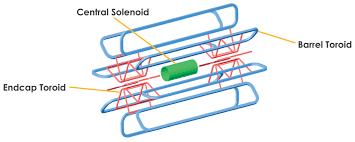
\includegraphics[width=0.5\textheight]{tesi_images/magnet_system_atlas.png}
				\caption{ATLAS magnet system}
			\end{figure}
			\begin{itemize}
				\item a solenoid, which is aligned on the beam axis and provides a $2$ T axial magnetic field for the inner detector,  while minimising the radiative thickness in front of thebarrel electromagnetic calorimeter;
				\item a  barrel  toroid and  two  end-cap  toroids, which  produce  atoroidal magnetic field of approximately $0.5$ T and $1$ T for the muon detectors in the centraland end-cap regions, respectively.
			\end{itemize}
			\subsection{Inner detector}
			The ATLAS Inner Detector (ID) is the inner-most ATLAS layer and it is immersed in a 2 T solenoidal field. It is designed to provide hermetic and robust pattern recognition, excellent momentum resolution and both primary and secondary vertex measurements forcharged tracks, with a lower limit in $p_t$  (nominally 0.5 GeV, but as low as 0.1 GeV) and within the pseudorapidity range $|\eta|<2.5$. It also provides electron identification over $|\eta|<2.0$ and a wide range of en-ergies (between 0.5 GeV and 150 GeV). \cite{ATLAS config}
			
			\begin{figure}
				\centering
				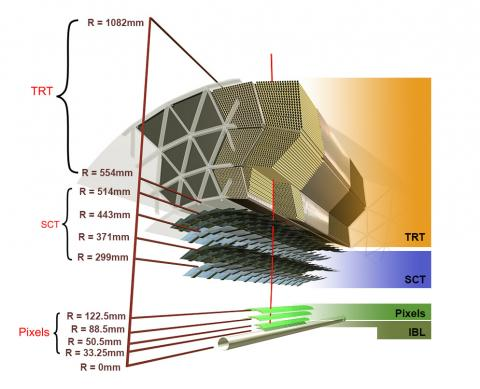
\includegraphics[width=0.3\textheight]{tesi_images/ID_structure.jpg}
				\caption{ATLAS Inner Detector structure}
			\end{figure}
			
			ID is composed by three independent but complementary sub-detectors: 
			\begin{itemize}
				\item  Pixel Detector:  \cite{Inner Detector}
				it is  the  inner-most  part  of  the  ATLAS  tracking  system. It consists of 4 layers of barrel pixel detector and two end caps of three pixel disks each. The innermost pixel layer is a high-resolution pixel detector,  called Insertable B-Layer (IBL). The Pixel Detector sits inside the 2T solenoidal magnetic field and contributes to the charged particle tracking of the ATLAS Inner Detector in the pseudo rapidity range of $|\eta|<2.5$. Due to its high spatial resolution and 3-dimensional space-point measurement the Pixel Detector has a key-role in reconstruction of charged particle tracks.  The 4-Layer Pixel Detector will be crucial in the reconstruction of primary and secondary vertices which is essential for the detection of long-lived particles.
				\item Semiconductor Tracker (SCT): \cite{SCT}
				it consists of 61 $m^2$ of active silicon-strip detector modules and it is immersed in a 2 T solenoidal magnetic field. The  SCT  covers  the  radial  region  from  30  to  52  cm,  with  hermetic  azimuthal  coverage  out  to $|\eta|=2.5$. Four cylindrical layers in the central region form the “barrel” detector, and nine annulardisks on each end of the barrel form the “endcaps”. The layout has been designed so that energetic charged particles will pass through at least four layers everywhere in the acceptance region.
				\item Transition Radiation Tracker (TRT): \cite{TRT}
				it is the outmost f the three tracking subsystems of the ATLAS Inner Detector. TRT s  a  straw-tube  tracker and it  consists  of  drift  tubes with a diameter of 4 mm that are made from wound Kapton and reinforced with thin carbon fibres. \\
				When a charged particle traverses the TRT, it ionises the gasinside the straws. The resulting free electrons drift towards thewire, where they are amplified and read out. \\
				The spaces between the straws are filled with polymer fibres(barrel) and foils (endcaps) to create transition radiation, whichmay be emitted by highly relativistic charged particles as theytraverse a material boundary.   This effect depends on the rel-ativistic factor $\gamma=E/m$ and is strongest for electrons.
				This design  makes the TRT complementary to  the silicon-based tracking devices:  the intrinsic single-point resolution of 120 $\mu$m is larger than that of the silicon trackers, but this is compensated by the large number of hits per track (typically morethan 30) and the long lever arm.  Furthermore, the high sam-pling frequency of the wire signals enables the TRT to providetiming information on the nanosecond level.
				RIFAI MEGLIOOOOOOOO OOOOOOOOOOOO OOOOOOOOOOOO OOOOOOOOOOOO  OOOO\\OO OOOOOOOOOOOOOOOOO\\OOO OOOOOOOOOOO O  OOOOOOOOOOOOOOOOO\\OOOOOOOO
			\end{itemize}
			\subsection{Calorimetry system}
			Calorimeters measure the energy a particle loses as it passes through the detector, so the energy of all charged and neu-
			tral particles. It is usually designed to stop entire or “absorb” most of the particles coming from a collision, forcing them to deposit all of their energy within the detector. Calorimeters typically consist of layers of “passive” or “absorbing” high-density material interleaved with layers of an “active” medium such as solid lead-glass or liquid argon. Calorimeters can stop most known particles except muons and neutrinos.
			
			The components of the ATLAS calorimetry system are: \cite{Calorimetry}
			\begin{itemize}
				\item electromagnetic calorimetry:
				The main part of ATLAS EM calorimeter is alead–liquid argon (LAr) sampling detector with accordion-shaped electrodes and lead absorber plates over its full coverage. The calorimeter isdivided into a Barrel part and two End-Caps (seeTable 1). Each End-Cap is divided into two coaxial wheels: an outer wheel and an inner wheelcovering, respectively, 1:375ojZjo2:5 and 2:5o. The absorber lead thickness is constantover large areas. The argon gap thickness isconstant in the Barrel but changing with theradius in the End-Cap.There are three longitudinal samplings forjZjo2:5 and two for 2:5ojZjo3:2:. n the rangejZjo1:8;the calorimeter is precededby a presampler (see Table 1) to recover the energylost in the upstream material (cryostat, super-conducting coil, inner detector, etc.). The activedepth of the presampler is 11 mm of liquid argonin the Barrel and 4 mm in the End-Cap.
				\item hadronic calorimeters:
				In the rangejZjo1:6;the ATLAS hadroniccalorimeter is an iron-scintillating tiles calorimeter.For rapidity larger than 1.6, the hadronic calori-meter is an LAr calorimeter. The Hadronic Tile calorimeter is located behindthe solenoid coil and the EM calorimeter. It is asampling calorimeter using iron as absorbermaterial and scintillating tiles as active material. The Hadronic End-Cap calorimeter (HEC) is anLAr sampling calorimeter which provides hadro-nic coverage for 1:5ojZjo3:2
				\item forward calorimeters (FCal):
				In the forward region (3:1ojZjo4:9), the EMcalorimetry is done by another type of LArcalorimeter. The Forward Calorimeter (FCAL)consists of copper rods parallel to the beam axisinside an outer tube with 250mm liquid argon gapin between
			\end{itemize}
		
		
			\subsection{Muon spectrometer}
			The  muon  spectrometer  forms  the  outer  part  of  the  ATLAS  detector  and  is  designed  to  detectcharged particles exiting the barrel and end-cap calorimeters and to measure their momentum inthe pseudorapidity range$|\eta|<2.7$.  It is also designed to trigger on these particles in the region$|\eta|<2.4$.
			
	
\newpage

	\chapter{Electron and photon reconstruction}
		Events with electrons and photons in the final state are important signatures for many physics analyses envisagedat the LHC. Their reconstruction mainly  exploits data coming from the electromagnetic calorimeter (clusters) and the Inner Detector (ID) systems (tracks) \cite{El ph intro}: 
		\begin{itemize}
			\item an electron is defined as an object consisting of a cluster built from energy deposits in the
			calorimeter (supercluster) and a matched track (or tracks);
			\item a  converted photon is a cluster matched to a conversion vertex (or vertices), and an unconverted photon is a cluster matched to neither an
			electron track nor a conversion vertex. About 20\% of photons at low $|\eta|$ convert in the ID, and up to about 65\% convert at $|\eta| \simeq 2.3$.
		\end{itemize}
		The reconstruction  with $|\eta| < 2.5$ is based on an algorithm. It first prepares the tracks and clusters it will use. It selects clusters of energy deposits measured in topologically connected EM and hadronic calorimeter cells, denoted topo-clusters. These clusters are matched to ID tracks, which are re-fitted accounting for bremsstrahlung. The algorithm also builds conversion vertices and matches them to the selected topo-clusters. The electron and photon supercluster-building steps then run separately using the matched clusters as input. After applying initial position corrections and energy
		calibrations to the resulting superclusters, the supercluster-building algorithm matches tracks to the electron superclusters and conversion vertices to the photon superclusters. The electron and photon
		objects to be used for analyses are then built, their energies are calibrated, and discriminating
		variables used to separate electrons or photons from background are added.
		
		\section{The topo-cluster reconstruction}
			The topo-cluster reconstruction algorithm begins by forming proto-clusters in the EM and hadronic calorimeters using a set of noise thresholds in which the cell initiating the cluster is EM required to have significance $|\zeta_{cell}^{EM}| \geq 4$ where 
			$$
			\zeta_{cell}^{EM} = \frac{E_{cell}^{EM}}{\sigma_{cell}^{EM}}
			$$		
			$E_{cell}^{EM}$ is the energy cell at the EM scale and $\sigma_{cell}^{EM}$ is the expected cell noise, which includes the known electronic noise and an estimate of the pile-up noise corresponding
			to the average instantaneous luminosity expected for Run 2. In order to suppres the formation of noise cluster, in this initial stage, cells from the presampler and the first LAr EM calorimeter layer are excluded from initiating proto-clusters.
			An important role is played by the neighbouring cells. If they have a significance $|\zeta_{cell}^{EM}| \geq 2$, these cells are collected by proto-cluster. Each neighbour cell passing the threshold of $|\zeta_{cell}^{EM}| \geq 2$ becomes a seed cell in the next iteration, collecting each of its neighbours in the proto-cluster. If two proto-clusters EM contain the same cell with $|\zeta_{cell}^{EM}| \geq 2$ above the noise threshold, these proto-clusters are merged. A crown of nearest-neighbour cells is added to the cluster independently on their energy ($|\zeta_{cell}^{EM}| \geq 0$). This set of thresholds is commonly known as ‘4-2-0’ topo-cluster reconstruction.\\
			Energy becomes an important feature when a cell has $|E_{cell}^{EM}| > 500$ MeV. A cell with this energy, at least four neighbours, and when none of the neighbours has a larger signal, is a local maximum. Proto-clusters with two or more local maxima are split into separate clusters.
			
			%Electron and photon reconstruction starts from the topo-clusters but only uses the energy from cells in the EM calorimeter, except in the transition region of $1.37<|\eta|<1.63$, where the energy measured in the presampler and the scintillator between the calorimeter cryostats is also added.%
		
		\section{Track reconstruction}
		Track finding is one of the most challenging tasks in reconstructing events from proton-proton  collisions  recorded  by  the  ATLAS  detector. The process consists in finding a track in the ID which can be matched to the energy clusters. The ID track reconstruction consists of several sequences with different strategies and the main sequence is referred to as inside-out track finding: \cite{ID reco alg}
		\begin{itemize}
			\item \textbf{Space point formation}: the initial step of the ID reconstruction consists of the cluster and drift circle creation and the transformation of clusters in the silicon detectors into 3D space points. Clusters are formed by finding connected cells in
			the pixel and strip detectors. \cite{Track reco}From these clusters, three-dimensional measurements referred to as space-points are created. In the pixel detector, each cluster equates to one space-point, while in the SCT, clusters from both stereo views of a strip layer must be combined to obtain a three-dimensional measurement. 
			
			\item \textbf{Space point seeded track finding}: track seeds are formed from sets of three space-points in the silicon-detector layers. \cite{ID reco alg} Seeds can be built from space points in the pixel detector only (referred to as PPP seeds), the strip detector only (SSS) or any mixed setup (PSS,PPS). To reduce the number of potential seeds, initial cuts are applied and dedicated care is taken not to
			extensively use space points in multiple seeds. Seeds that pass the initial requirements are then input to a track finding algorithm that uses a combinatorial Kalman filter technique and aims to complete the track candidates within the silicon detector.
			
			\item \textbf{Ambiguity solving}: track candidates are then further processed in an ambiguity solving
			module that aims to eliminate track candidates from random hit combinations (often
			referred to as "fakes") or track duplicates, which can be identified by measurements that are shared with other track candidates. The ambiguity solving relies on a scoring function applying positive scores for unique measurements and good fit quality, while penalising missing measurements where they would be expected (also called holes) or shared measurements with other track candidates.
			
			\item \textbf{TRT extension}: tracks that successfully pass the ambiguity solving stage and are within the coverage of the TRT detector are then extended into the TRT and completed for measurements in the outermost tracking detector. A successful TRT extension increases the
			momentum resolution significantly by exploiting the longer lever arm for field integration.
		\end{itemize}
		
		\section{Track-cluster matching and photon conversion reconstruction}

		\section{Supercluster reconstruction}
		The reconstruction of electron and photon superclusters proceeds independently, each in two stages \cite{El ph reco}:
		\begin{enumerate}
		\item in the first stage, EM topo-clusters are tested for use as seed cluster candidates, which form the basis of superclusters; 
		\item in the second stage, EM topo-clusters near the seed candidates are identified as satellite cluster candidates, which may emerge from bremsstrahlung radiation or topo-cluster splitting.
		\end{enumerate}
		Superclusters are built through various steps:
		\begin{itemize}
		\item the initial list of EM topo-clusters is
		sorted according to descending $E_T$ , calculated using the EM energy.
		\item the clusters are tested one by one in the sort order for use as seed clusters. There are two seed's kind:
			\begin{enumerate}[label=\roman*.]
				\item electron supercluster seed: a cluster with a minimum $E_T$ of 1 GeV and matched to a track with at least four hits in the silicon tracking detectors.
				\item photon supercluster seed: a cluster with $E_T$ greater
				than 1.5 GeV with no requirement made on any track or conversion
				vertex matching.
			\end{enumerate}
		A cluster cannot be used as a seed cluster if it has already been added as a satellitecluster to another seed cluster.
		\item if a cluster meets the characteristics of the previous point, the algorithm attempts to find satellite clusters, using the process summarized in figure \ref{fig:super_cl}.
		\begin{figure}
			\centering
			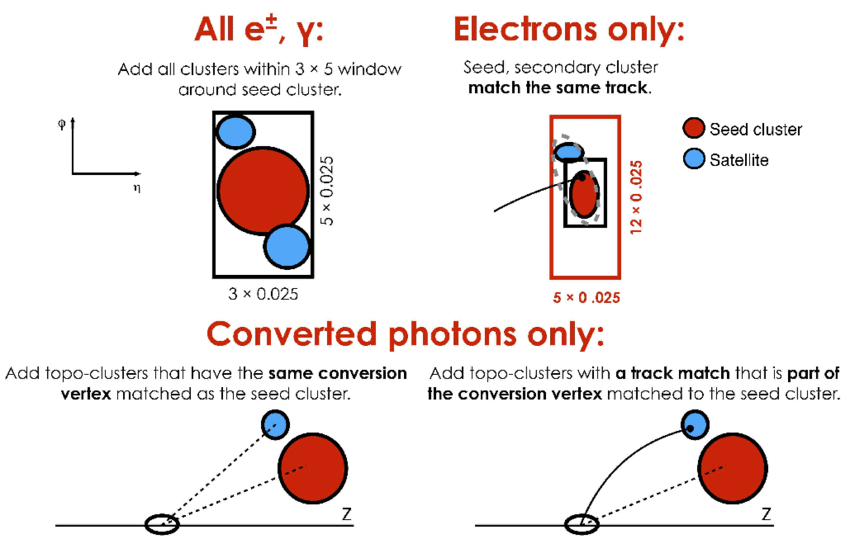
\includegraphics[width=0.45\textheight]{tesi_images/super_cluster.png}
			\caption{Diagram of the superclustering algorithm for electrons and photons. Seed clusters are shown in
			red, satellite clusters in blue.}
			\label{fig:super_cl}
		\end{figure}
		For both electrons and photons, a cluster is considered a satellite if it falls within a window of $\Delta\eta \times \Delta\varphi = 0.075 \times 0.125$ around the seed cluster barycentre, as these cases tend to represent secondary EM showers originating from the same initial electron or photon.
		For electrons, this window could be larger, $\Delta\eta \times \Delta\varphi = 0.125 \times 0.300$, and its ‘best-matched’ track is also the best-matched track for the seed cluster. For photons with conversion vertices made up only of tracks containing silicon hits, a cluster is added as a satellite if its best-matched (electron) track belongs to the conversion vertex matched to the seed cluster. These steps rely on tracking information to discriminate distant radiative photons or conversion electrons from pile-up noise or other unrelated clusters. \\
		The seed clusters with their associated satellite clusters are called superclusters.
		
		\item The final step in the supercluster-building algorithm is to assign calorimeter cells to a given supercluster. Only cells from the presampler and the first three LAr calorimeter layers are considered, except in the transition region of $1.4 < |\eta| < 1.6$, where the energy measured in the scintillator between the calorimeter cryostats is also added. To limit the superclusters’ sensitivity to pile-up noise, the size of each constituent topo-cluster is restricted to a maximal width of 0.075 or 0.125 in the $\eta$ direction in the barrel or endcap region, respectively. Because the magnetic field in the ID is parallel to the beam-line, interactions between the electron or photon and detector material generally cause the EM shower to spread in the $\varphi$ direction, so the restriction in $\eta$ still generally allows the electron or photon energy to be captured. No restriction is applied in the $\varphi$-direction.	
		\end{itemize}
		\section{Creation of electrons and photons for analysis}
		\cite{El ph reco}After the electron and photon superclusters are built, tracks are matched to electron superclusters and conversion vertices to photon superclusters. Then the analysis-level
		electrons and photons are created. Because electron and photon superclusters are built independently, a given seed cluster can produce both an electron and a photon. In such cases, the procedure
		presented in figure \ref{fig:el_ph_analisi} is applied. The purpose is that if a particular object can be easily identified only as a photon (a cluster with no good track attached) or only as an electron (a cluster with a good track attached and no good photon conversion vertex), then only a photon or an electron object is created for analysis; otherwise, both an electron and a photon object are created. Furthermore,these cases are marked explicitly as ambiguous, allowing the final classification of these objects to be determined based upon the specific requirements of each analysis.
		\begin{figure}
			\centering
			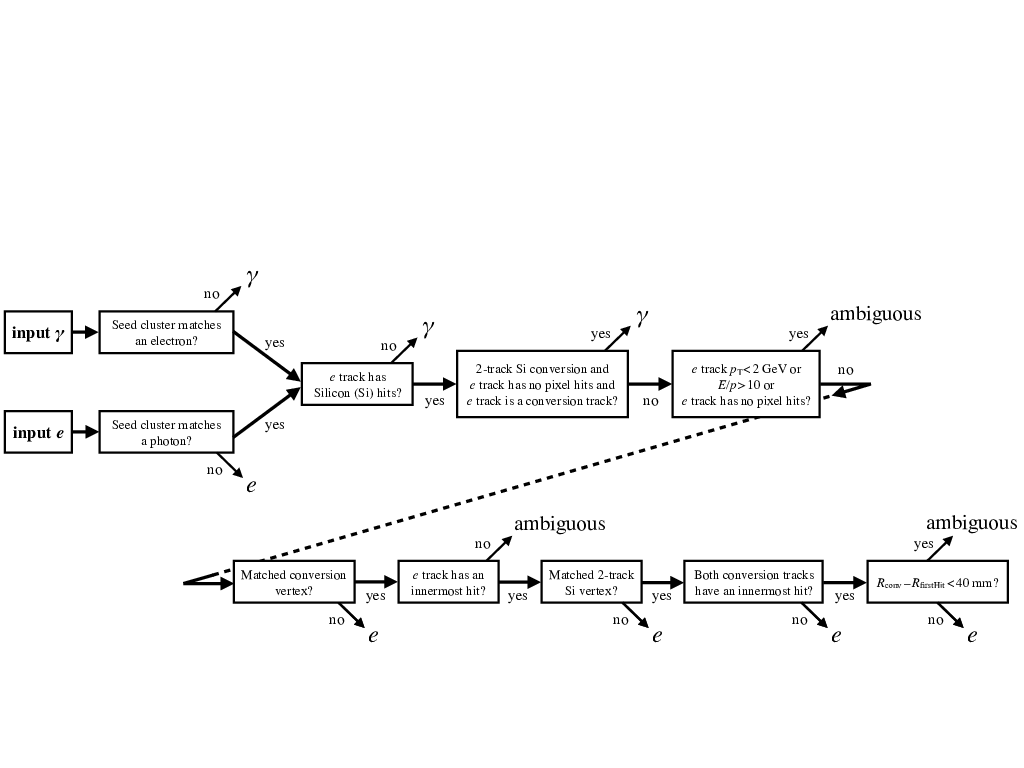
\includegraphics[width=0.45\textheight]{tesi_images/el_ph_analisi.png}
			\caption{Flowchart showing the logic of the ambiguity resolution for particles initially reconstructed both as electrons and photons.}
			\label{fig:el_ph_analisi}
		\end{figure}
	
		\section{Identification}
		\cite{Identification}Excellent electron and photon identification capabilities are crucial for many aspects of the ATLAS physics program, from standard model measurements (including Higgs boson) to new physics searches. The identification of prompt photons and the rejection of backgrounds, mostly coming from photons from hadron decays, relies on the high granularity of the ATLAS calorimeter. Electron identification is based on a likelihood (LH) discrimination to separate isolated electron candidates from candidates originating from photon conversions, hadron misidentification and heavy flavor decays. 
			\subsection{Elettron identification}
			\cite{El ph reco}The quantities used in the electron identification are chosen according to their ability to discriminate prompt isolated electrons from energy deposits from hadronic jets, from converted photons and from genuine electrons produced in the decays of heavy-flavour hadrons. The variables can be
			grouped into properties of:
			\begin{itemize}
				\item the primary electron track, which is required to fulfil a set of quality requirements, namely hits in the two inner tracking layers closest to the beam line, as well as a number of hits in the silicon-strip detectors. The transverse impact parameter of the track and its significance are used to construct
				the likelihood discriminant.
				\item the lateral development of the electromagnetic shower, which is characterized with variables calculated separately in the first and second layer of the electromagnetic calorimeter. To reject clusters from multiple incident particles, $w_{s tot}$ is used. The lateral shower development is measured with $R_{\varphi}$ and $R_{\eta}$.
				\item the longitudinal development of the electromagnetic shower, for them the numbers of cells contributing to the energy
				measurement in each layer are chosen dynamically in the supercluster approach, compared with fixed numbers of cells in fixed-size clusters. The supercluster approach inherently suppresses noise in the calorimeter cells, resulting in lower values and narrower distributions. The electron
				identification uses $f_1$ and $f_3$.
				\item the spatial compatibility of the primary electron track with the reconstructed cluster, which are matched using $\Delta\eta_1$ and $\Delta\phi_{res}$. 
			\end{itemize}
			\begin{figure}
				\centering
				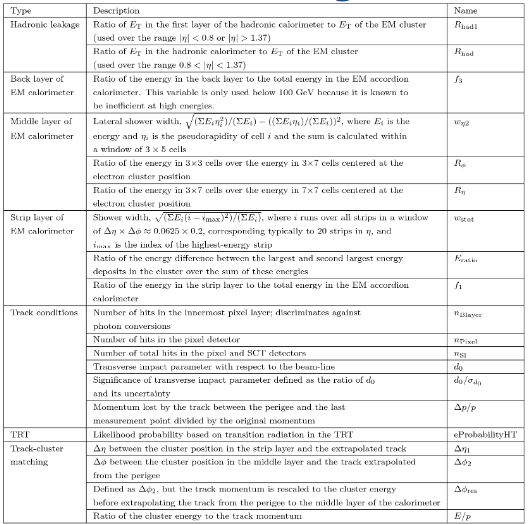
\includegraphics[width=0.45\textheight]{tesi_images/el_discr.png}
				\caption{Electron discriminating variables}
				\label{fig:el_discr}
			\end{figure}
			Then the combination of information from the tracker and the matching, information from the electromagnetic calorimeter, and hadronic leakage  are put together in likelihoods for a reconstructed electron to originate from signal,
			$L_S$, or background, $L_B$. They are calculated from probability density functions (pdfs), $P$:
			$$
			L_{S/B}(\textbf{x}) = \prod_{i=1}^{n}P_{S/B,i}(x_i)
			$$
			For signal and background the pdfs take the values $P_{S,i}(x_i)$ and $P_{B,i}(x_i)$, respectively, for the quantity $i$ at value $x_i$. The likelihood discriminant $d_L$ is defined as the natural logarithm of the ratio of $L_S$ and $L_B$:
			$$
			d_L = \ln{\frac{L_S}{L_B}}
			$$
			and each electron is assigned a specific value.\\
			Using the same variables but different values of $d_L$, three different operating points: Loose, Medium and Tight. They are sorted with increasing threshold values, and are chosen in order to have efficiency for electrons with $E_T > 40$ GeV of 93\%, 88\%, and 80\% respectively. This means that they are inclusive, and one the subset of the other.
			
			\subsection{Photon identification}
			\cite{El ph reco}The photon identification criteria are designed to efficiently select prompt, isolated photons and reject backgrounds from hadronic jets. The photon identification is constructed from one-dimensional
			selection criteria, or a cut-based selection, using the shower shape variables. AGGIUNGERE TABELLA VARIABILI
			The variables using the EM first layer play a particularly important role in rejecting $\pi^0$ decays into
			two highly collimated photons. The primary identification selection is labelled as Tight, with less restrictive selections called
			Medium and Loose, which are used fo the $R_{had}$, $R_{had_1}$, $R_{\eta}$, and $w_{\eta_2}$ shower shape variables. The Medium selection adds a loose cut on $E_{ratio}$. Because the reconstruction of photons in the ATLAS trigger system does not differentiate between converted and unconverted photons, the Loose and Medium identification criteria are the same for converted
			and unconverted photons. The Tight identification criteria are designed to select a subset of the photon candidates passing the Medium criteria.\\
			Because the shower shapes vary due to the geometry of the calorimeter, the cut-based selection of Loose, Medium and Tight
			are optimized separately in bins of $|\eta|$. The Tight identification is also optimized in separate bins of $E_T$. The Tight identification is performed separately for converted and
			unconverted photons. The shower shapes of converted photons differ from unconverted photons due to the opening angle of the $e^{+}e^{-}$ conversion pair, which is amplified by the magnetic field, and from the additional interaction of the conversion pair with the material upstream of the calorimeters. \\
			The tight selections are separately optimised for unconverted and converted photons, to account for the generally broader lateral shower profile of the latter. The thresholds of the selection criteria are different in seven intervals of the reconstructed photon $|\eta|$ to account for the calorimeter geometry, and for different effects on the shower shapes from the material upstream of the calorimeter.
			
		\section{Electron and photon isolation}
		The isolation progress, or isolation cut, is applied in order to reduce the backgrounds. Different criteria are defined, with different levels
		of efficiency in rejecting the background. The isolation working points uses variables from the tracking and from the calorimeter.
		
		\cite{El ph reco}The activity near leptons and photons can be quantified from the tracks of nearby charged particles, or from energy deposits in the calorimeters, leading to two classes of isolation variables:
		\begin{itemize}
			\item The raw calorimeter isolation($E_{T,raw}^{isol}$) is built by summing the transverse energy of positive-energy topological clusters (in EM scale) whose barycentre falls within a cone centred around the electron or photon cluster barycentre. The raw calorimeter isolation includes the EM particle energy ($E_{T,core}$), which is subtracted by removing the energy of the EM calorimeter cells contained in a $\Delta\eta \times \Delta\varphi = 5 \times 7$ (in EM-middle-layer units) rectangular
			cluster around the barycentre of the EM particle cluster. Other correction are done to account for the pile-up. %(using MC samples)%
			
			The fully corrected calorimeter isolation variable is computed as:
			$$ 
			E_{T}^{coneXX} = E_{T,raw}^{isolXX} - E_{T}^{core} - E_{T,leakage}(E_T,\eta,\Delta R) -E_{T,pile-up}(\eta,\Delta R)
			$$
			where XX refers to the size of the employed cone.
			\item The track isolation variable ($p_T^{coneXX}$) is computed by summing the transverse momentum of selected tracks within a cone centred around the electron track or the photon cluster direction (excluding tracks matched to the electron or converted photon). \cite{El ph isol}In order to compensate for very busy environment at high $p_T$ the cone is of variable size:
			$$
			\Delta R = min\Bigl({\frac{10}{p_T[GeV]},\Delta R_{max}}\Bigr)
			$$
			where $\Delta R_{max}$ is the maximum cone size (typically 0.2).
			
			The tracks considered are required to have $p_T >$ 1 GeV and $|\eta| <$ 2.5, at least seven silicon (Pixel + SCT) hits, at most one shared hit, at most two silicon holes and at most one pixel hole. In addition, for electron isolation, the tracks are required to have a loose vertex association, i.e. the track was used in the primary vertex fit, or it was not used in any vertex fit but satisfies $|\Delta z_0|sin{\theta} < 3$ mm, where $|\Delta z_0|$ is the longitudinal impact parameter relative to the chosen primary vertex; for photon
			isolation, all selected tracks satisfying $|\Delta z_0|sin{\theta} < 3$ mm are used.
		\end{itemize}
		
		
		
		
		
	\chapter{Machine Learning}
		Machine Learning (ML) as been instrumental for the advances of both data analysis and artificial intelligence (AI) \cite{Lifelong ML}. ML is an application of AI with the aim of generating systems with the ability to automatically learn and improve from experience without being explicitly programmed. The ML algorithm is exposed to a training dataset in order to generate a mathematical model,which is then applied in real-life performance tasks. %(it is used for making predictions).
		
		ML can be divided into three main categories \cite{ML categories}:
		\begin{enumerate}
			\item \textbf{Supervised Learning}: the goal is to learn a mapping from inputs \textbf{x} to outputs $y$, given a labeled set of input-output pairs $D = \{(x_i, y_i)\}_{i=1}^{N}$. Here $D$ is called the training set, and $N$ is the number of training examples. In the simplest setting, each training input $\textbf{x}_i$ is a $D$-dimensional vector of numbers, which are called features, attributes or covariates. In general, however, $\textbf{x}_i$ could be a complex structured object.
			
			The form of the output or response variable can in principle be anything, but most methods assume that $y_i$ is a categorical or nominal variable from some finite set, $y_i \epsilon  \{1, . . . , C\}$ or that $y_i$ is a real-valued scalar. When $y_i$ is categorical, the problem is known as classification or pattern recognition, and when $y_i$ is real-valued, the problem is known as regression.
			
			\item \textbf{Unsupervised learning}: here to the algorithm is only given inputs, $D = \{(x_i)\}_{i=1}^{N}$, and the goal is to find “interesting patterns” in the data. This is sometimes called knowledge discovery. %This is a much less well-defined problem, since we are not told what kinds of patterns to look for, and there is nocobvious error metric to use (unlike supervised learning, where we can compare our prediction of y for a given x to the observed value).%
			
			\item \textbf{Reinforcement learning}: this is useful for learning how to act or behave when given occasional reward or punishment signals. A reinforcement learning algorithm, or agent, learns by interacting with its environment. The agent receives rewards by performing correctly and penalties for performing incorrectly. The agent learns without intervention from a human by maximizing its reward and minimizing its penalty.
			
		\end{enumerate}
		\section{Supervised Learning}
		Let's focus on the supervised learning. \cite{GBT}
			\subsection{Model and Parameters}
			As written above, the model in supervised learning usually refers to the mathematical structure of by which the prediction $y_i$ is made from the input $\textbf{x}_i$.
		
			The parameters are the undetermined part that we need to learn from data. In linear regression problems, the parameters are the coefficients $\theta$. Usually $\theta$ is used to denote the parameters (there are many parameters in a model).
		
			\subsection{Objective Function}
			In order to train the model, we need to define the a function of the parameters to measure how well the model fit the training data. This function is called: \textit{Objective function}.
			
			A characteristic of objective functions is that they are composed of two parts (also dependent on parameters): training loss $L$ and regularization term $\Omega$:
			$$
			obj(\theta) = L(\theta) + \Omega(\theta)
			$$
			The training loss measures how predictive our model is with respect to the training data. Common choices of $L$ are the mean squared error, which is given by:
			$$
			L(\theta) = \sum_{i}(y_i - y_{i_{pred}})^2
			$$
			or logistic loss, to be used for logistic regression:
			$$
			L(\theta) = \sum_{i}  [{ y_i\ln(1+e^{-y_{i_{pred}}}) + (1-y_i) \ln(1+e^{-y_{i_{pred}}})    }]
			$$
			
			The regularization term controls the complexity of the model, which helps to avoid overfitting. The general principle is a simple and predictive model. The tradeoff between the two is also referred as bias-variance tradeoff in machine learning.
		\section{Gradient boosted trees}
		There are many models, which ML algorithms can use, and one of them is a
		Decision Tree ensemble. If it is trained, it becomes a Gradient Boosted Tree. The basic unit is decision tree.
			\subsection{Decision Tree}
			Decision Trees (DTs) are a supervised learning method used for classification and regression.
			\cite{Decision Tree}A decision tree is a hierarchical structure consisting of nodes and directed edges. The tree has three types of nodes:
			\begin{itemize}
				\item a root node that has no incoming edges and zero or more outgoing edges.
				\item internal nodes, each of which has exactly one incoming edge and two or more outgoing edges.
				\item leaf or terminal nodes, each of which has exactly one incoming edge and no outgoing edges.
			\end{itemize}
			
			\subsection{Decision Tree Ensembles}
			\cite{GBT}The tree ensemble model consists of a set of classification and regression trees (CART). A CART is a bit different from decision trees, in which the leaf only contains decision values. In CART, a real score is associated with each of the leaves. This also allows for a principled, unified approach to optimization.
			
			Usually, a single tree is not strong enough to be used in practice. So the ensemble model is used. In this model the prediction scores of each individual tree are summed up to get the final score:
			$$
			y_{i_{pred}} = \sum_{k=1}^{K} f_k(x_i), f_k \epsilon \mathcal{F}
			$$
			where $K$ is the number of trees, $f$ is a function in the functional space $\mathcal{F}$, and $\mathcal{F}$ is the set of all possible CARTs. The objective function to be optimized is given by:
			$$
			obj(\theta)
			$$
			
		\section{LightGBM}
		
		
		
		
		
	\begin{thebibliography}{17}
			
			%%%%%%%%%%%%%%%%%%%%%%%%%%%%%%%%%%%%%%%%%%%%%%%%%%%%%%%%%%%%%%%%%%%%%%%%%%%%%%%%%%%%%%%%%%%%%%%%%%%%%%%%%%%%%%%%%%%%%%%%%%%%%%%%%%%%%%%%%%%%%%%%%%%%%%%%%%%%%%%%%%%%%%%%%%%%%%%%%%%%%%%%%%%%%%%%%%%%%%%%%%%%%%%
			%\textbf{\Large Chapter 2} 
			
			% 1 %
			\bibitem{LHC design} European organization for nuclear research, \textit{LHC design report}, CERN libraries, Geneva (2004). \url{http://cds.cern.ch/record/782076/files/}
			% 2 %
			\bibitem{LHC introduction} F. Gianotti, \textit{Collider physics: LHC}, EP Division, CERN, Geneva, Switzerland. \url{https://cds.cern.ch/record/458489/files/p219.pdf}
			% 3 % 
			\bibitem{Acc. complex} \url{https://cds.cern.ch/record/2255762/files/CERN-Brochure-2017-002-Eng.pdf}
			% 4 %
			\bibitem{ATLAS intro} \url{https://home.cern/science/experiments/atlas}
			% 5 % 
			\bibitem{ATLAS config}  The ATLAS Collaboration et al 2008 JINST3 S08003
			\url{https://iopscience.iop.org/article/10.1088/1748-0221/3/08/S08003/pdf}
			% 6 % 
			\bibitem{Inner Detector} H. Pernegger, \textit{The Pixel Detector of the ATLAS Experiment for LHC Run-2}, ATL-INDET-PROC-2015-001. \url{https://cds.cern.ch/record/1985432/files/ATL-INDET-PROC-2015-001.pdf}
			% 7 %
			\bibitem{SCT} J.R. Pater \textit{The ATLAS SemiConductor Tracker operation and performance}, 2012 JINST7 C04001. \url{https://iopscience.iop.org/article/10.1088/1748-0221/7/04/C04001/pdf}
			% 8 % 
			\bibitem{TRT} Adrian Vogel \textit{ATLAS Transition Radiation Tracker (TRT): Straw Tube Gaseous Detectors at High Rates}, CERN,
			Geneva, ATL-INDET-PROC-2013-005, Apr 2013, ATL-INDET-PROC-2013-005. \url{https://cds.cern.ch/record/1537991}
			% 9 %v
			\bibitem{Calorimetry}
			\url{http://ific.uv.es/~cabrera/teaching/atlas_i.pdf}\\
			
			%%%%%%%%%%%%%%%%%%%%%%%%%%%%%%%%%%%%%%%%%%%%%%%%%%%%%%%%%%%%%%%%%%%%%%%%%%%%%%%%%%%%%%%%%%%%%%%%%%%%%%%%%%%%%%%%%%%%%%%%%%%%%%%%%%%%%%%%%%%%%%%%%%%%%%%%%%%%%%%%%%%%%%%%%%%%%%%%%%%%%%%%%%%%%%%%%%%%%%%%%%%%%%%
		 	\textbf{\Large Chapter 2} 
		 	
			% 10 %
			\bibitem{El ph intro} Wu Xin, Clark Allan and Campanelli Mario \textit{Electron and photon identification in ATLAS}, Springer Berlin Heidelberg, Berlin, Heidelberg, 2006
			\url{https://link.springer.com/chapter/10.1007/978-3-540-32841-4_21} 
			% 11 %
			\bibitem{El ph reco}
			\textit{Electron and photon performance measurements with the {ATLAS} detector using the 2015-2017 {LHC} proton-proton collision data}
			\url{https://iopscience.iop.org/article/10.1088/1748-0221/14/12/P12006}
			% 12 %
			\bibitem{In-out alg} \textit{A neural network clustering algorithm for the ATLAS silicon pixel detector}, The ATLAS collaboration
			\url{{https://doi.org/10.1088%2F1748-0221%2F9%2F09%2Fp09009}}
			% 13 % 
			\bibitem{Track reco}
			\url{https://link.springer.com/content/pdf/10.1140/epjc/s10052-019-7140-6.pdf}in
			% 14 % 
			\bibitem{ID reco alg} \textit{Optimisation of the ATLAS Track Reconstruction Software for Run-2}, Andreas Salzburger, CERN, Switzerland, \url{http://iopscience.iop.org/1742-6596/664/7/072042}
			% 15 % 
			\bibitem{Identification} \textit{Electron and photon identification with the ATLAS detector}, Proklova Nadezda, ATLAS Collaboration, Aug 2018, ATL-PHYS-SLIDE-2018-606, \url{http://cds.cern.ch/record/2634679}
			% 16 %
			\bibitem{El ph isol} \textit{SEARCH FOR SUPERSYMMETRY WITH A COMPRESSED MASS SPECTRUM USING THE ATLAS DETECTOR}, Rossini Lorenzo, \url{http://hdl.handle.net/2434/683343 }\\
			
			%%%%%%%%%%%%%%%%%%%%%%%%%%%%%%%%%%%%%%%%%%%%%%%%%%%%%%%%%%%%%%%%%%%%%%%%%%%%%%%%%%%%%%%%%%%%%%%%%%%%%%%%%%%%%%%%%%%%%%%%%%%%%%%%%%%%%%%%%%%%%%%%%%%%%%%%%%%%%%%%%%%%%%%%%%%%%%%%%%%%%%%%%%%%%%%%%%%%%%%%%%%%%%%
			\textbf{\Large Chapter 3}
			
			% 17 %
			\bibitem{Lifelong ML} \textit{Lifelong Machine Learning}, Zhiyuan Chen and Bing Liu, Morgan \& Claypool Publishers, Nov 2016, \url{https://www.cs.uic.edu/~liub/lifelong-machine-learning-draft.pdf}
			% 18 %
			\bibitem{ML categories} \textit{Machine Learning: A Probabilistic Perspective}, Kevin P. Murphy, The MIT Press, \url{https://scholar.google.it/scholar?q=K.P.+Murphy,+Machine+Learning.+A+Probabilistic+Perspective+,+MITpress+(2012)&hl=it&as_sdt=0&as_vis=1&oi=scholart}
			% 19 % 
			\bibitem{GBT} \url{https://xgboost.readthedocs.io/en/latest/tutorials/model.html}
			% 20 %
			\bibitem{Decision Tree} \textit{4Classification:Basic Concepts,Decision Trees, andModel Evaluation}, \url{https://www-users.cs.umn.edu/~kumar001/dmbook/ch4.pdf}
	\end{thebibliography}
\end{document}